\chapter{Design and Implementation}

\section{Design Approach}

There are several methods that can be used to detect a signal as listed in~\cite{riviello2013sensing}. One of the methods is energy detection, which is the most popular method due to its simplicity. Energy detection works by considering the power level of the signal captured by receive. If the power level drops below a certain threshold value, the detector will not detect the signal. Otherwise, the signal will be categorized as detected signal. The power level of the signal is obtained from FFT, which then squared and averaged to get the magnitude. This value will be compared with the threshold value. Note that in order to get a stable signal, the detector is equipped with moving average filter after getting the magnitude. In addition, band-pass filter is used right before FFT calculation to reduce noise. The block diagram of the proposed detector can be seen in Figure~\ref{fig:block-diagram}

\begin{figure}[h]
	\centering
    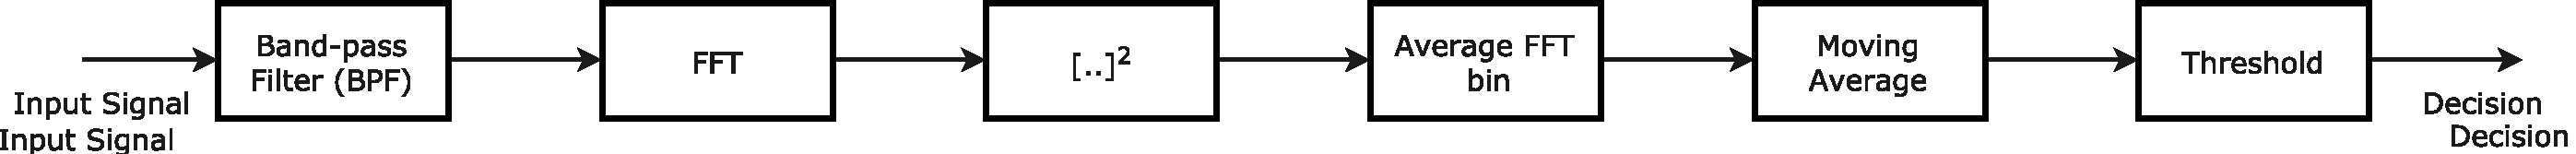
\includegraphics[width=\textwidth]{figures/block-diagram}
    \caption{Proposed energy detector block diagram}
    \label{fig:block-diagram}
\end{figure}

From~\cite{radiotvnederland}, a DVB-T carrier frequency has 8 MHz bandwidth, which can contain up to 12 channels depending on the modulation and also the quality of the channels. As we do not consider modulation and demodulation method for this project, the decision process works by only considering the bandwidth. For instance, if the detector detects a signal beyond $\pm$8 MHz, it will not be categorized as detected DVB-T signal. Using such approach gives a trade-off between misdetection and false alarm. Most likely, it reduces the probability of false alarm but may lead to the increased probability of misdetection.  However, the main advantage is that the detector supposedly can distinguish between DVB-T signal and other signals.

\section{Implementation in GNU Radio}

In this project, the detector is built using SDR dongle, Realtek RTL2832U, which is used as a receiver. The dongle is capable of capturing FM, DVB-T, and DAB signal. It has a built-in band-pass filter to eliminate undesired frequencies. The signal that has been filtered will be converted to digital data using A/D converter and ready to be processed afterwards. We use GNU Radio Companion to process the captured signal. GNU Radio Companion allows us to easily build functional block diagrams but lacks of features for testing or building automated test scenario. Luckily, GNU Radio Companion generates a Python script, which can be run through GNU Radio Companion GUI or terminal just like running ordinary Python script. The script can be modified or imported to a new python script in which the automation functions reside. We prefer to create a new python script, called 'main' function because the generated script will be replaced once the block diagram is modified~\cite{gnuradio2016,alexandrucsete2011,sivantoledo2012}. The block diagram of the proposed detector created using GNU Radio Companion can be seen in Figure~\ref{fig:gnuradio-block-diagram} along with its description in Table~\ref{tbl:gnu-diagram-block}.

\begin{figure}[h]
    \centering
    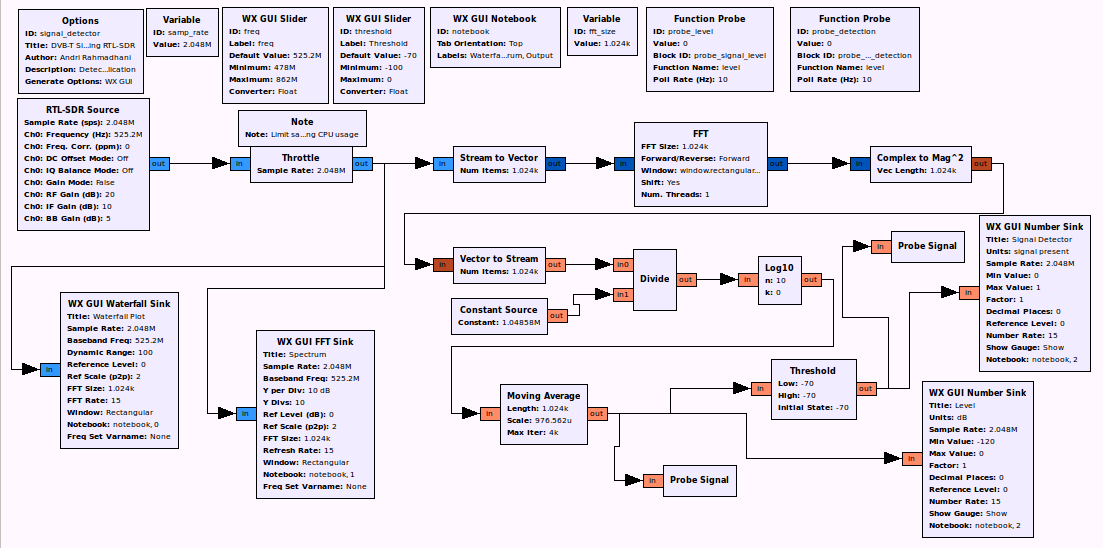
\includegraphics[width=\textwidth]{figures/gnuradio-block-diagram}
    \caption{Diagram block of proposed detector in GNU Radio Companion}
    \label{fig:gnuradio-block-diagram}
\end{figure}

The block diagram is built based on the workflow of the detector as seen in Figure~\ref{fig:workflow}. First, the main python script is executed. The script has a feature to let user inputs command parameters. Then, the GUI generated by GNU Radio Companion will appear and the automated measurement start running. The script will run automatic noise level finder to obtain and set appropriate threshold if it is specified in input parameters. Subsequently, the script will incrementally scan frequencies in the given range, or the given list read from a file depending on the input parameters. In the scanning process, if the power level is higher than the threshold, the detection status is set to true (1) otherwise is set to false (0). The results are saved to files for further processing.

\begin{figure}[h]
    \centering
    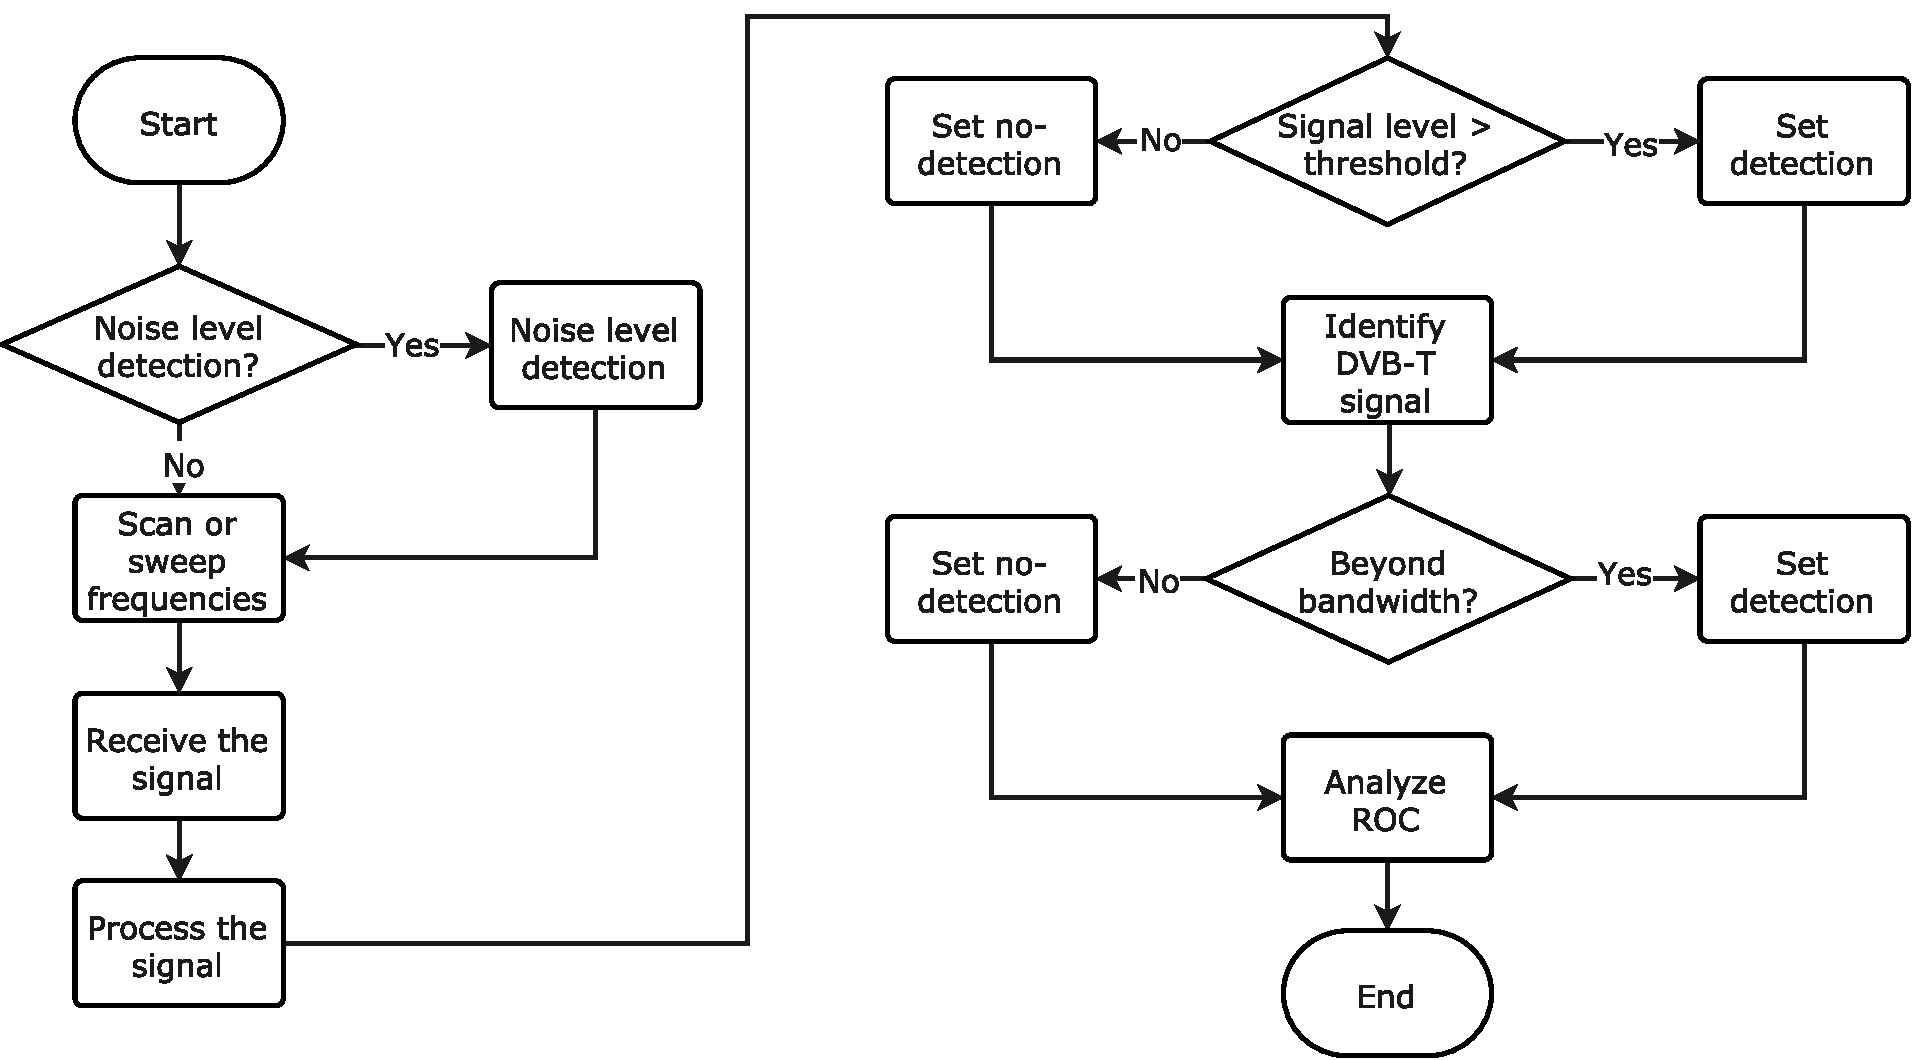
\includegraphics[width=0.9\textwidth]{figures/workflow}
    \caption{Workflow of proposed detector}
    \label{fig:workflow}
\end{figure}

In order to improve the detection results, we introduce DVB-T signal identifier to distinguish between DVB-T and other signals based on bandwidth. It counts the number of consecutive detections in a certain range of frequency and tries to find the center frequency by taking the median. If the detection is far beyond the bandwidth, the detector decides not to raise the detection flag. Otherwise, the detector set the detection flag to true (1), indicating the presence of DVB-T signal. The results will be used to analyze Receiver Operating Characteristic (ROC), which can be done automatically using the Python script~\cite{matplotlib2016,scipy.org2015,justinjohnson2016}.

\begin{table}[h]
\centering
\caption{GNU Radio block diagram description}
\label{tbl:gnu-diagram-block}
\resizebox{\textwidth}{!}{%
\begin{tabular}{|p{0.2\textwidth}|p{0.4\textwidth}|p{0.4\textwidth}|}
\hline
\multicolumn{1}{|c|}{\textbf{Block Name}} & \multicolumn{1}{c|}{\textbf{Description}}                                                                                                   & \multicolumn{1}{c|}{\textbf{Parameter}}                                                                  \\ \hline \hline
RTL-SDR Source                            & Getting the input of signal from RTL2838 dongle                                                                                             & \makecell[lt]{Sample Rate : 2.048 M Samples/s \\ RF Gain : 20 dB \\ IF Gain : 10 dB \\ Baseband Gain : 5 dB \\ BW : 1 MHz} \\ \hline
Throttle                                  & Limiting the sample per sec (sampling rate)                                                                                                 & Sample Rate : 2.048 M Samples/s                                                                          \\ \hline
Stream to Vector                          & Converting stream data into vector in order to be processed in FFT                                                                          & Num Items : fft\_size (1024)                                                                             \\ \hline
Complex to Mag\textasciicircum 2          & Calculating magnitude squared value of FFT sample output                                                                                    &                                                                                                          \\ \hline
Vector to Stream                          & Converting Vector to Stream after FFT process. (The opposite of Stream to Vector block)                                                     & Num Items : fft\_size (1024)                                                                             \\ \hline
Constant Source                           & Generating (FFT size) 2 value as a divisor                                                                                                  & (fft\_size) 2                                                                                            \\ \hline
Divide                                    & Getting the average bins of FFT Result (Complex to Mag\textasciicircum 2) by (FFT size) 2 in order to get the power                         &                                                                                                          \\ \hline
Log10                                     & Converting the power level into dB P (dB) = 10*log(P {[}Watt{]})                                                                            &                                                                                                          \\ \hline
WX GUI FFT Sink (Spectrum)                & Displaying FFT results of spectrum                                                                                                          & \makecell[lt]{Sample Rate : 2.048 M Samples/s \\ Baseband freq : freq \\ FFT Size : fft\_size (1024) \\ Window : Rectangular} \\ \hline
WX GUI Waterfall Sink                     & Displaying waterfall spectrogram                                                                                                            & \makecell[lt]{Sample Rate : 2.048 M Samples/s \\ Baseband freq : freq \\ FFT Size : fft\_size (1024) \\ Window : Rectangular} \\ \hline
WX GUI Number Sink (Level)                & Displaying the level value in dB                                                                                                            & \makecell[lt]{Sample Rate : 2.048 M Samples/s \\ Min value : -120 \\ Max value : 0 \\ Average Alpha : 0.03}                   \\ \hline
Threshold                                 & Setting the threshold with upper limit -60 dB                                                                                               & threshold                                                                                                \\ \hline
WX GUI Number Sink (Signal Detection)     & Displaying the signal detection based on threshold set. “1” if there is a signal present and “0” if there is no signal present              & \makecell[lt]{Sample Rate : 2.048 M Samples/s \\ Min value : 0 \\ Max value : 1}                                            \\ \hline
Variable Sampling Rate                    & Define the sampling rate                                                                                                                    & samp\_rate : 2.048 M Sample/s                                                                            \\ \hline
Variable FFT Size                         & Define the FFT Size                                                                                                                         & fft\_size : 1024                                                                                         \\ \hline
WX GUI Slider Frequency                   & Define the frequency                                                                                                                        & \makecell[lt]{freq \\ freq. min : 478 MHz \\ req. max : 862 MHz}                                                            \\ \hline
WX GUI Slider Threshold                   & Define the threshold. It will give “1” if the signal level is above -60 dB and will give “0” if the signal level is below -60 dB.           & \makecell[lt]{threshold \\ default = -60 dB \\ min : -100 dB \\ max : 0 dB}                                                   \\ \hline
Probe Signal                              & Probe output of a block                                                                                                                     & ID : probe\_signal\_level                                                                                \\ \hline
Probe Signal                              & Probe output of a block                                                                                                                     & ID : probe\_signal\_detection                                                                            \\ \hline
Function Probe                            & Allow a probe signal to be accessible in Python script. It can be used to get output value of a block in which the probe signal is attached & \makecell[lt]{ID : probe\_level \\ Block ID : probe\_signal\_level \\ Function Name : level}                                \\ \hline
Function Probe                            & Allow a probe signal to be accessible in Python script. It can be used to get output value of a block in which the probe signal is attached & \makecell[lt]{ID : probe\_detection \\ Block ID : probe\_signal\_detection \\ Function Name : level}                        \\ \hline
Moving Average                            & Applying Moving Average to stabilized data                                                                                                  & \makecell[lt]{Length : fft\_size \\ Scale: 1.0/fft\_size}                                                                 \\ \hline
\end{tabular}%
}
\end{table}